\chapter{Horizonte, Zustandsgleichung und Vakuumenergie}

\section{Bevorzugtes Bezugssystem, überlichtschnelle Entfernung und Horizont}

Der kosmische Mikrowellenhintergrund zeichnet tatsächlich ein spezielles Bezugssystem aus. In dem Bezugssystem, in dem diese Strahlung isotrop erscheint, sind im Mittel auch die nahen Galaxien in Ruhe. Bewegen wir uns durch den Hintergrund, werden Photonen in Bewegungsrichtung zu höheren Energien und Photonen in Gegenrichtung zu niedrigeren Energien Doppler-verschoben. Das bevorzugte Bezugssystem ist dasjenige, in dem der Mikrowellenhintergrund isotrop erscheint; zugleich ist es im Mittel das Bezugssystem, in dem die lokalen Galaxien in Ruhe sind.

\begin{classroomqa}\lecturetimestamp{00:00:25}\audiencequestion{Hängt die scheinbare Wellenlänge der kosmischen Strahlung von der Bewegung des Beobachters ab, und bedeutet das, dass es ein bevorzugtes Bezugssystem gibt?}\lecturerresponse{Ja. Die Bewegung durch den Mikrowellenhintergrund erzeugt eine Doppler-Anisotropie. Daher gibt es ein bevorzugtes kosmologisches Bezugssystem: dasjenige, in dem der Mikrowellenhintergrund isotrop erscheint. Zugleich ist es im Mittel das Bezugssystem, in dem die lokalen Galaxien in Ruhe sind.}\end{classroomqa}

Eine zweite Frage betrifft die Fluchtgeschwindigkeiten. Nach dem Hubble-Gesetz entfernen sich hinreichend weit entfernte Galaxien voneinander gemäß
\begin{equation}
v = H d .
\end{equation}
Für hinreichend große \(d\) übersteigt diese Fluchtgeschwindigkeit die Lichtgeschwindigkeit. Das widerspricht der Relativitätstheorie nicht, denn das Verbot gilt lokal: Kein Objekt kann unmittelbar vor uns schneller als das Licht an einem anderen vorbeiziehen. Die Aussage über weit entfernte Galaxien betrifft die Geometrie zwischen weit voneinander entfernten Orten.

\begin{classroomqa}\lecturetimestamp{00:04:48}\audiencequestion{Können zwei Galaxien eine Relativgeschwindigkeit haben, die größer ist als \(c\)?}\lecturerresponse{Ja, wenn sie weit genug voneinander entfernt sind. Die Hubble-Flucht kann die Lichtgeschwindigkeit überschreiten, ohne der lokalen Relativitätstheorie zu widersprechen. Der Ort, an dem die Fluchtgeschwindigkeit \(c\) erreicht, ist ein Horizont.}\end{classroomqa}

Sobald die Fluchtgeschwindigkeit die Lichtgeschwindigkeit erreicht, machen Signale, die auf uns zu gesendet werden, keinen Nettfortschritt mehr. Der Lichtstrahl bewegt sich lokal weiterhin mit der Grenzgeschwindigkeit, aber die zu überwindende Entfernung wächst zu schnell.

\begin{classroomqa}\lecturetimestamp{00:07:03}\audiencequestion{Würde ein Lichtstrahl, der in die entgegengesetzte Richtung ausgesandt wird, sich nicht trotzdem auf uns zubewegen?}\lecturerresponse{Lokal tut er das, aber der Raum wächst schneller, als der Strahl die Entfernung überwinden kann. Der Strahl bewegt sich relativ zu benachbarten Punkten mit der Grenzgeschwindigkeit, während die Gesamtentfernung zu uns weiter zunimmt.}\end{classroomqa}

\section{Die expandierende Metrik und die Analogie mit einer Linie}

Ein anschauliches Bild ergibt sich in einer Dimension. Stellen wir uns eine Linie aus Atomen vor. Dehnen wir eine gewöhnliche materielle Linie, reißt sie irgendwann. Ändern wir nun das Bild: Immer wenn sich benachbarte Atome zu weit voneinander entfernen, fügen wir ein weiteres Atom dazwischen ein. Die Linie wächst weiter, aber ihre lokalen Eigenschaften dünnen nicht aus.

\begin{figure}\centering
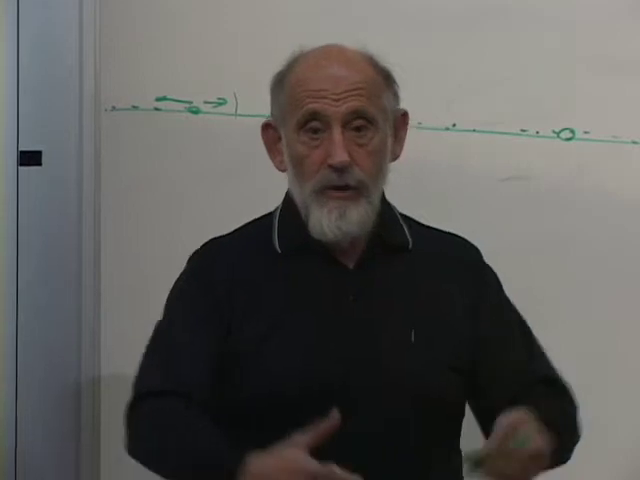
\includegraphics[width=0.60\textwidth]{lecture_04_figure_02.png}\caption{Eindimensionale Linie zur Veranschaulichung einer expandierenden Metrik.}\end{figure}

In diesem Bild gibt es weiterhin eine lokale Grenzgeschwindigkeit für Signale, so wie Schall auf einer gewöhnlichen Linie eine Grenzgeschwindigkeit hat. Die Regel gilt lokal: Eine Störung kann sich relativ zu benachbarten Punkten nicht schneller ausbreiten. Ist die Linie jedoch lang genug und werden schnell genug neue Punkte eingefügt, entfernen sich weit genug voneinander entfernte Teile so rasch, dass ein Signal niemals zurückgelangen kann.

Die relativistische Geschwindigkeitsaddition ist daher nur ein Teil der Geschichte. Sie gilt lokal, wenn Beobachter am selben Ort aneinander vorbeiziehen. Für weit voneinander entfernte Galaxien in einer expandierenden Geometrie ist sie nicht das geeignete Werkzeug.

\begin{classroomqa}\lecturetimestamp{00:09:42}\audiencequestion{Gilt in dieser Situation weiterhin das gewöhnliche relativistische Gesetz für die Addition von Geschwindigkeiten?}\lecturerresponse{Lokal, an einem Ort, ja. Ziehen Beobachter nacheinander aneinander vorbei, gilt die gewöhnliche spezielle relativistische Regel. Sie eignet sich jedoch nicht zur Beschreibung der Flucht weit voneinander entfernter Galaxien mit mehr als \(c\); dafür muss man auf die Geometrie des expandierenden Raums zurückgreifen.}\end{classroomqa}

Dasselbe Bild liefert eine einfache Erklärung der Rotverschiebung. Zeichnet man eine Welle auf die Linie, wächst ihre Wellenlänge mit der Linie mit, wenn diese expandiert. In einer expandierenden Geometrie ist das nicht bloß ein anschauliches Bild. Wellengleichungen in der expandierenden Raumzeit ergeben tatsächlich gestreckte Wellenlängen.

\begin{classroomqa}\lecturetimestamp{00:14:42}\audiencequestion{Ist die Aussage, dass sich eine Welle mit dem Universum ausdehnt, theoretisch, empirisch oder beides?}\lecturerresponse{Sie folgt theoretisch aus der Wellenausbreitung in der expandierenden Raumzeit und wird außerdem durch astronomische Beobachtungen gestützt.}\end{classroomqa}

Dieses Bild ist kein Gummiband. Ein Gummiband wird beim Dehnen dünner, und jemand, der in einem solchen Medium lebt, würde Veränderungen der lokalen Eigenschaften feststellen. Hier bleiben die lokalen Eigenschaften gleich, während der globale Maßstab der Entfernungen wächst.

\section{Letzte Streuung und das beobachtbare Universum}

Der Horizont ist der Ort, an dem die Fluchtgeschwindigkeit die Lichtgeschwindigkeit erreicht. Die Oberfläche der letzten Streuung liegt knapp innerhalb davon. Ein Signal, das vom Horizont ausgesandt würde, wäre unbeschränkt rotverschoben; die Strahlung der letzten Streuung weist eine enorme, aber endliche Rotverschiebung auf.

\begin{classroomqa}\lecturetimestamp{00:17:53}\audiencequestion{Wie hängen überlichtschnelle Flucht, die Oberfläche der letzten Streuung und das beobachtbare Universum zusammen?}\lecturerresponse{Der Horizont ist der Ort, an dem die Fluchtgeschwindigkeit die Lichtgeschwindigkeit erreicht. Die Oberfläche der letzten Streuung liegt knapp innerhalb davon, da ihre Rotverschiebung enorm, aber endlich ist. Praktisch gesehen markiert sie den Rand des beobachtbaren Universums.}\end{classroomqa}

Die Rotverschiebung der Strahlung von der letzten Streuung beträgt ungefähr den Faktor \(10^3\). Dieser Wert ist bereits so groß, dass die Oberfläche der letzten Streuung für viele Zwecke sehr nahe am Horizont liegt. Das beobachtbare Universum ist der Teil des Universums, aus dem Licht uns erreichen kann.

Zu späten Zeiten nähert sich die Expansion dem vakuumdominierten Regime. Dann strebt die Hubble-Größe einem konstanten Wert zu, der Horizont nähert sich einer festen Größe, und sowohl Galaxien als auch Mikrowellenstrahlung verschwinden nach und nach aus unserem Blickfeld.

\begin{classroomqa}\lecturetimestamp{00:22:43}\audiencequestion{Da sich \(H\) mit der Zeit ändert, ändert sich dann auch die Horizontentfernung, und wird der Mikrowellenhintergrund irgendwann verschwinden?}\lecturerresponse{Zu späten Zeiten strebt \(H\) einem konstanten Wert zu, sodass sich der Horizont einer festen Entfernung nähert. Der Mikrowellenhintergrund wird weiterhin gedehnt, kühlt ab und verblasst. Auch weit entfernte Galaxien überschreiten den Horizont und verschwinden aus unserem Blickfeld.}\end{classroomqa}

Sichtbar bleiben nur Strukturen, die bereits gravitativ gebunden sind. Das Sonnensystem fliegt nicht auseinander, und auch die Galaxie fliegt nicht auseinander, doch das Universum wird im großen Maßstab zu einer isolierten Insel.

\section{Die grundlegende Expansionsgleichung und die drei Komponenten}

Die grundlegende Expansionsgleichung lautet nun
\begin{equation}
\left(\frac{\dot a}{a}\right)^2 = \frac{8\pi G}{3}\rho ,
\qquad c=1 .
\end{equation}
Dabei ist \(a(t)\) der Skalenfaktor und \(\rho\) die Gesamtenergiedichte.

\begin{figure}\centering
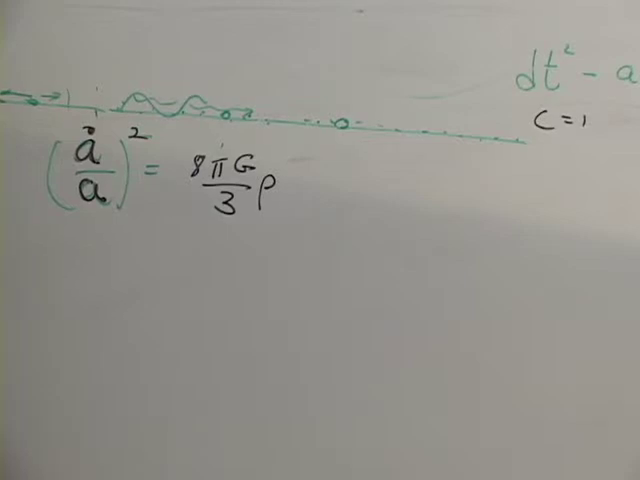
\includegraphics[width=0.74\textwidth]{lecture_04_figure_03.png}\caption{Grundlegende Expansionsgleichung und Analogie mit der eindimensionalen Linie.}\end{figure}

Drei Komponenten sind dynamisch bedeutsam.

Für Materie gilt
\begin{equation}
\rho=\frac{\text{const.}}{a^3},
\qquad
a(t)\sim t^{2/3}.
\end{equation}
Das ist der Fall massiver Objekte, die sich mit der Gesamtexpansion bewegen und im mitbewegten Bezugssystem im Wesentlichen in Ruhe sind.

Für Strahlung gilt
\begin{equation}
\rho=\frac{\text{const.}}{a^4},
\qquad
a(t)\sim t^{1/2}.
\end{equation}
Die zusätzliche Potenz von \(a\) ergibt sich daraus, dass jedes Photon bei der Expansion des Universums rotverschoben wird.

Außerdem gibt es
\begin{equation}
\rho_0=\text{constant},
\end{equation}
die Vakuumenergie, auch dunkle Energie genannt oder, bis auf übliche numerische Faktoren, die kosmologische Konstante. Diese Komponente verdünnt sich überhaupt nicht.

Als Nächstes muss die Energiedichte mit dem Druck in Beziehung gesetzt werden.

\section{Strahlungsdruck und kalte Materie}

Beginnen wir mit Strahlung. Betrachten wir einen eindimensionalen Kasten, also einfach ein Liniensegment der Länge \(L\), in dem Photonen hin und her reflektiert werden. In einer Dimension sind Kraft und Druck praktisch dasselbe.

Betrachten wir ein Photon mit dem Impulsbetrag \(p\). Bei der Reflexion an einer Wand ändert sich sein Impuls um
\begin{equation}
\Delta p = 2p.
\end{equation}
Die Zeit zwischen zwei aufeinanderfolgenden Stößen an derselben Wand beträgt
\begin{equation}
\Delta t = \frac{2L}{c}.
\end{equation}
Die mittlere Kraft auf die Wand ist daher
\begin{equation}
F=\frac{\Delta p}{\Delta t}=\frac{pc}{L}.
\end{equation}
Für ein Photon gilt
\begin{equation}
E=pc,
\end{equation}
also
\begin{equation}
F=\frac{E}{L}.
\end{equation}
Die Energie geteilt durch die Länge ist die eindimensionale Energiedichte. In diesem eindimensionalen Fall gilt
\begin{equation}
P=\rho .
\end{equation}

Bei vielen Photonen bleibt derselbe Zusammenhang nach der Mittelung erhalten. Die Gesamtkraft entspricht einfach der Gesamtenergie pro Längeneinheit.

Gehen wir nun zu drei Dimensionen über. Bewegten sich alle Photonen nur entlang einer Achse, würden sie Druck auf ein Paar von Flächen ausüben und auf die übrigen Flächen keinen. Das ist bewusst falsch angesetzt, zeigt aber unmittelbar, was korrigiert werden muss. In einem isotropen Strahlungsbad ist der Impuls auf alle Richtungen verteilt. Im Mittel trägt ein Drittel der Energiedichte zu jeder Druckkomponente bei. Das Ergebnis lautet
\begin{equation}
P=\frac{\rho}{3}.
\end{equation}

Für kalte Materie fällt das Ergebnis anders aus. Betrachten wir einen mitbewegten Kasten, also ein kleines Gebiet, das sich mit der Strömung des Universums bewegt. Die Teilchen darin tragen Energie, aber wenn sie relativ zum Kasten in Ruhe sind, stoßen sie nicht gegen seine Wände. Der Druck ist daher
\begin{equation}
P=0.
\end{equation}

\begin{figure}\centering
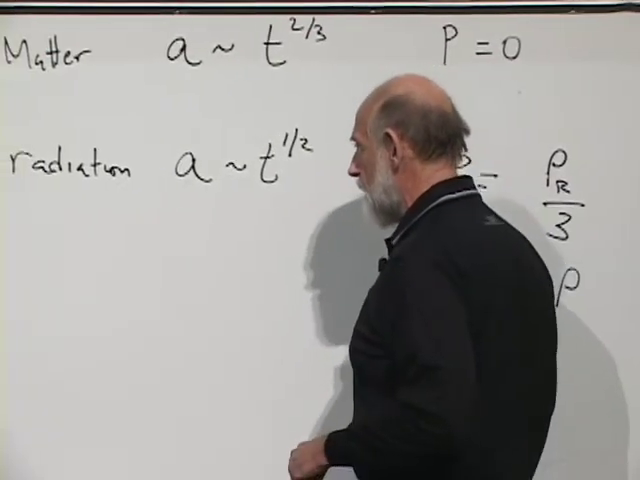
\includegraphics[width=0.74\textwidth]{lecture_04_figure_04.png}\caption{Materie und Strahlung: \(a\sim t^{2/3}\), \(P=0\) und \(a\sim t^{1/2}\), \(P=\rho/3\).}\end{figure}

Die Zusammenfassung an der Tafel lautet
\begin{align}
\text{matter:}\qquad & a(t)\sim t^{2/3}, \qquad P=0,\\
\text{radiation:}\qquad & a(t)\sim t^{1/2}, \qquad P=\frac{\rho}{3}.
\end{align}

\begin{classroomqa}\lecturetimestamp{00:54:27}\audiencequestion{Bewegen sich die Teilchen im expandierenden Universum nicht tatsächlich voneinander weg?}\lecturerresponse{Ja, aber die Druckbetrachtung bezieht sich auf einen infinitesimal kleinen mitbewegten Kasten. Auf dieser lokalen Skala gilt die thermodynamische Argumentation weiterhin.}\end{classroomqa}

\section{Die Zustandsgleichung}

Der Druck wird als proportional zur Energiedichte angenommen:
\begin{equation}
P=w\rho .
\end{equation}
An der Tafel wird derselbe Parameter mit \(\omega\) bezeichnet. Für die beiden grundlegenden Fälle gilt
\begin{equation}
w=0 \quad \text{for cold matter},
\qquad
w=\frac{1}{3} \quad \text{for radiation}.
\end{equation}

Auch Zwischenfälle sind möglich. Werte zwischen \(0\) und \(1/3\) beschreiben Materie, die weder vollständig kalt noch voll relativistisch ist. Als Beispiel wird hier warme dunkle Materie genannt.

\begin{figure}\centering
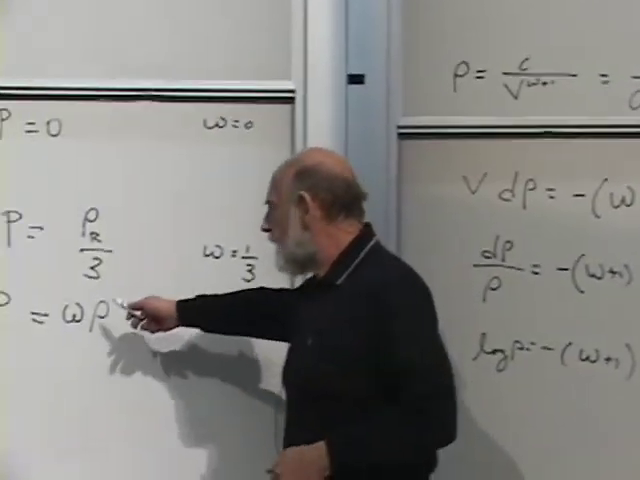
\includegraphics[width=0.74\textwidth]{lecture_04_figure_05.png}\caption{Zustandsgleichung \(P=\omega\rho\) zusammen mit der Herleitung der Skalierung der Dichte.}\end{figure}

Als Nächstes stellt sich die Frage, ob \(w\) die Abhängigkeit von \(\rho\) von \(a\) bestimmt. Die Antwort ergibt sich aus einer thermodynamischen Identität.

Betrachten wir einen Kasten mit Volumen \(V\). Übt der Inhalt einen Druck \(P\) aus, so verrichtet er bei einer Volumenzunahme des Kastens um \(dV\) an den Wänden die Arbeit
\begin{equation}
dE=-P\,dV.
\end{equation}
Schreiben wir nun die Energie als
\begin{equation}
E=\rho V.
\end{equation}
Ihr Differential lautet
\begin{equation}
dE=\rho\,dV+V\,d\rho .
\end{equation}
Setzt man die beiden Ausdrücke gleich, erhält man
\begin{equation}
\rho\,dV+V\,d\rho=-P\,dV,
\end{equation}
oder
\begin{equation}
V\,d\rho=-(\rho+P)\,dV.
\end{equation}
Mit \(P=w\rho\) folgt
\begin{equation}
V\,d\rho=-(1+w)\rho\,dV.
\end{equation}
Teilen wir durch \(\rho V\):
\begin{equation}
\frac{d\rho}{\rho}=-(1+w)\frac{dV}{V}.
\end{equation}
Durch Integration ergibt sich
\begin{equation}
\rho \propto V^{-(1+w)}.
\end{equation}
Für einen kosmologischen, mitbewegten Kasten gilt
\begin{equation}
V\propto a^3,
\end{equation}
und damit
\begin{equation}
\rho \propto a^{-3(1+w)}.
\end{equation}

Damit erhält man unmittelbar die zuvor betrachteten Fälle zurück:
\begin{align}
w=0 &\Longrightarrow \rho \propto a^{-3},\\
w=\frac{1}{3} &\Longrightarrow \rho \propto a^{-4}.
\end{align}

Deshalb ist \(w\) von Bedeutung. Sobald \(\rho(a)\) bekannt ist, kann man es wieder in die Friedmann-Gleichung einsetzen. Dann nimmt man ein Potenzgesetz \(a\sim t^\alpha\) an und bestimmt, wie sich das Universum für diese Zustandsgleichung ausdehnt.

\section{Vakuumenergie und negativer Druck}

Ein besonderer Fall verhält sich anders:
\begin{equation}
w=-1.
\end{equation}
Dann gilt
\begin{equation}
1+w=0,
\end{equation}
Der Exponent verschwindet also, und es gilt
\begin{equation}
\rho=\rho_0=\text{constant}.
\end{equation}
Der zugehörige Druck ist
\begin{equation}
P=-\rho .
\end{equation}

Negativer Druck ist an sich nicht rätselhaft. Positiver Druck drückt die Wände eines Kastens nach außen. Negativer Druck zieht sie nach innen. Er entspricht einer Spannung. Ein gedehntes Gummiband ist ein alltägliches Beispiel: Es speichert positive Energie, zieht seine Enden aber zusammen.

Setzen wir die konstante Dichte \(\rho_0\) in die Friedmann-Gleichung ein:
\begin{equation}
\left(\frac{\dot a}{a}\right)^2=\frac{8\pi G}{3}\rho_0.
\end{equation}
Die rechte Seite ist einfach eine Zahl, also gilt
\begin{equation}
\frac{\dot a}{a}=\sqrt{\frac{8\pi G}{3}\rho_0}.
\end{equation}
In diesem besonderen Fall ist die Hubble-Größe tatsächlich konstant. Die Gleichung lässt sich schreiben als
\begin{equation}
\dot a=\sqrt{\frac{8\pi G}{3}\rho_0}\,a,
\end{equation}
und die Lösung lautet
\begin{equation}
a(t)\propto \exp\!\left(\sqrt{\frac{8\pi G}{3}\rho_0}\,t\right).
\end{equation}

Das ist exponentielle Expansion. Die maßgebliche Zeitskala ist die \(e\)-fache Zeit, nicht die Verdopplungszeit; die hier verwendete grobe Abschätzung ordnet sie in die Größenordnung des Alters des Universums ein. Vakuumenergie und kosmologische Konstante bezeichnen denselben physikalischen Bestandteil, abgesehen von historischen Konventionen für numerische Faktoren.

\begin{classroomqa}\lecturetimestamp{01:27:16}\audiencequestion{Wenn Vakuumenergie exponentielle Expansion antreibt, wird dann nicht irgendwann alles auseinandergerissen?}\lecturerresponse{Nicht unbedingt. Gebundene Systeme können ihr widerstehen. Eine Galaxie, ein Sonnensystem oder ein Atom muss nicht auseinandergerissen werden, während hinreichend große und dünn verteilte Strukturen an der Expansion teilhaben und sich schließlich voneinander entfernen.}\end{classroomqa}

\begin{classroomqa}\lecturetimestamp{01:31:43}\audiencequestion{Hat das negative Vorzeichen beim Ziehen der Quadratwurzel aus der Friedmann-Gleichung eine interessante Bedeutung?}\lecturerresponse{Ja. Die Quadratwurzel liefert zwei Zweige. Einer ist die expandierende Lösung, der andere die zeitumgekehrte kontrahierende Lösung. Die Gleichungen selbst lassen beide zu.}\end{classroomqa}

\section{Drei Epochen und die beobachtete Expansionsgeschichte}

Alle drei Komponenten sind vorhanden und skalieren unterschiedlich:
\begin{equation}
\begin{aligned}
\rho_{\text{radiation}}&\propto a^{-4},\\
\rho_{\text{matter}}&\propto a^{-3},\\
\rho_0&=\text{constant}.
\end{aligned}
\end{equation}
Daraus folgen unmittelbar drei Epochen.

Bei sehr kleinem \(a\) dominiert die Strahlung. Später dominiert Materie. Bei hinreichend großem \(a\) dominiert die Vakuumenergie. Die zugehörigen Expansionsgesetze lauten
\begin{equation}
a(t)\sim t^{1/2},
\qquad
a(t)\sim t^{2/3},
\qquad
a(t)\sim e^{Ht}.
\end{equation}

Die hier genannten ungefähren Zeitpunkte sind folgende: Nach etwa \(10^4\) Jahren geht die Strahlungsdominanz in die Materiedominanz über. Später, nach etwa \(10^5\) Jahren, wird das Universum durchsichtig. Der Übergang von der Materiedominanz zur beschleunigten Expansion erfolgt viel später, nach mehreren Milliarden Jahren, in der hier verwendeten Größenordnungsschätzung ungefähr zur Halbzeit der kosmischen Geschichte.

Wie lässt sich diese Geschichte erschließen? Die Zukunft können wir nicht sehen, wohl aber die Vergangenheit. Größere Entfernung bedeutet, dass wir weiter in die Vergangenheit blicken. Indem man weit entfernte Galaxien beobachtet, misst, wie ihre Bewegung mit ihrer Entfernung zusammenhängt, und die Hubble-Größe als Funktion der Rückblickzeit rekonstruiert, lässt sich der zeitliche Verlauf des Skalenfaktors bestimmen. Die strahlungsdominierte Epoche liegt zu früh, um sie direkt mit gewöhnlicher Galaxienastronomie zu beobachten. Die materiedominierte Epoche und der Übergang zur Vakuumdominanz sind jedoch in der rekonstruierten Kurve sichtbar.

\section{Letzte Streuung in ferner Zukunft}

Der Mikrowellenhimmel in ferner Zukunft erzählt eine andere Geschichte als Galaxien, die den Horizont überschreiten. Die Strahlung, die wir zu späteren Zeiten sehen, stammt von weiter entfernter Materie. Der Effekt besteht also darin, weiter und kühler in die Tiefe des Universums zu blicken, und nicht darin, dass dieselben Atome einfach immer weiter davonfliegen.

\begin{classroomqa}\lecturetimestamp{01:48:07}\audiencequestion{Wenn die Oberfläche der letzten Streuung im Horizont verblasst, ist das dasselbe wie Galaxien, die sich über den Horizont hinausbewegen?}\lecturerresponse{Nein. Die spätere Strahlung stammt nicht von denselben Atomen wie die Strahlung, die wir jetzt sehen. Sie stammt von Atomen, die weiter entfernt waren. Es ist, als blickte man immer tiefer in das Universum, während die Strahlung immer kühler erscheint.}\end{classroomqa}

\section{Krümmung, das Bild des Big Crunch und der Horizont zu späten Zeiten}

Bislang wurde der Krümmungsterm weggelassen. Nimmt man ihn wieder hinzu, ergibt sich
\begin{equation}
\left(\frac{\dot a}{a}\right)^2
=
\frac{8\pi G}{3}\rho
-
\frac{K}{a^2}.
\end{equation}
Numerisch scheint dieser Term klein zu sein, begrifflich ist er jedoch wichtig. In der älteren Newtonschen Sprache unterscheidet er Fälle positiver, verschwindender und negativer Gesamtenergie. In der relativistischen Sprache unterscheidet er die räumlichen Geometrien.

Bevor Vakuumenergie ernst genommen wurde, stellte man sich häufig ein materiedominiertes Universum vor, in dem sich die Expansion schließlich umkehren würde. Daraus ergab sich das alte Bild des Big Crunch: Expansion nach dem Urknall, gefolgt von einer erneuten Kontraktion. Die Mathematik gilt weiterhin, scheint aber unser Universum nicht mehr zu beschreiben.

\begin{classroomqa}\lecturetimestamp{01:53:51}\audiencequestion{Hängt diese Vakuumenergie mit der quantenmechanischen Vakuumenergie zusammen?}\lecturerresponse{Ja, oder zumindest glaubt man das.}\end{classroomqa}

Die ungefähre Zusammensetzung heute ist
\begin{equation}
\frac{\rho_0}{\rho_{\text{total}}}\sim 0.7,
\qquad
\frac{\rho_{\text{matter}}}{\rho_{\text{total}}}\sim 0.3.
\end{equation}
Von der Materiekomponente entfallen etwa \(0.05\) der Gesamtmenge auf leuchtende Materie und etwa \(0.25\) auf dunkle Materie. Strahlung ist heute vernachlässigbar. Dunkle und leuchtende Materie skalieren gleich, daher bleibt ihr Verhältnis konstant, auch wenn sich die relativen Anteile von Materie, Strahlung und Vakuum von Epoche zu Epoche ändern.

Im vakuumdominierten Grenzfall gilt
\begin{equation}
H=\sqrt{\frac{8\pi G}{3}\rho_0}.
\end{equation}
Dann wird das Hubble-Gesetz zu
\begin{equation}
v=Hd.
\end{equation}
Der Horizont ist durch \(v=1\) definiert, seine Entfernung beträgt also
\begin{equation}
d_H=\frac{1}{H}
=
\frac{1}{\sqrt{8\pi G\rho_0/3}}.
\end{equation}
Die hier genannte grobe Größenordnung liegt bei \(10\) bis \(12\) Milliarden Lichtjahren.

Entscheidend ist das Verhalten zu späten Zeiten. Sobald die Expansion exponentiell verläuft, wird die Horizontentfernung konstant. Galaxien überschreiten ihn weiterhin und verschwinden, indem sie immer stärker rotverschoben werden. Auch der Mikrowellenhintergrund wird immer weiter rotverschoben. In ferner Zukunft bleiben nur die nahen gravitativ gebundenen Strukturen sichtbar, und das Universum erscheint wie eine isolierte Insel.

\section{Geometrie anhand der Oberfläche der letzten Streuung}

Schließlich lässt sich die Geometrie anhand der Oberfläche der letzten Streuung prüfen. Nehmen wir an, die Entfernung zu dieser Oberfläche sei bekannt. Nehmen wir außerdem an, man könne dort eine Verdichtung ausmachen, deren physikalische Größe hinreichend genau bekannt ist. Dann kann man diese Größe und Entfernung mit der beobachteten Winkelausdehnung vergleichen.

In einem flachen Raum entspricht der Winkel dem euklidischen Wert. In einem positiv gekrümmten Raum erschiene das Objekt größer, in einem negativ gekrümmten kleiner. Die Analogie ist eine gewöhnliche Vermessung: Man nimmt ein Objekt bekannter Größe in bekannter Entfernung und vergleicht den gemessenen Winkel mit dem Wert, den die euklidische Geometrie vorhersagt.

\begin{classroomqa}\lecturetimestamp{02:08:09}\audiencequestion{Was ist ein Beispiel für ein Objekt dort draußen, dessen Größe wir kennen?}\lecturerresponse{Die größten Verdichtungen im Mikrowellenhintergrund. Wir glauben, ihre Größe aus der Zeit, die sie für ihre Entwicklung benötigten, und aus der Schallgeschwindigkeit zu kennen.}\end{classroomqa}

Hier geht es um die größten Verdichtungen im Mikrowellenhintergrund. Ihre beobachtete Winkelausdehnung stimmt bis auf wenige Prozent mit der euklidischen Geometrie überein. Auf dieser Grundlage erscheint der Raum flach.

\section{Gemessenes \(w\) und eine abschließende Frage}

Die Beobachtungsbedeutung von \(w\) ist nun klar. Wenn Astronomen berichten, dass \(w\) sehr nahe bei \(-1\) liegt, sagen sie damit, dass die Vakuumenergiekomponente nahezu konstant ist. Genau das ist der hier dargelegte Punkt.

Das bedeutet nicht, dass die allgemeine Relativitätstheorie \(w\) zwingend genau auf \(-1\) festlegt. Hier geht es um eine empirische Aussage. In der Vorlesung wird kurz erwähnt, dass grundsätzlich auch radikalere Möglichkeiten nicht ausgeschlossen sind. Für den Fall einer nahezu konstanten Vakuumenergie gibt es jedoch gute Gründe, ihn für plausibel zu halten.

\begin{classroomqa}\lecturetimestamp{02:11:04}\audiencequestion{Haben wir bei der Berechnung der Dichte für Materie und Strahlung angenommen, dass die Energie konstant ist, und dann den Skalenfaktor angepasst, um die Formel zu bestimmen? Und falls das für die ersten beiden Fälle gilt: Was geschieht dann im Fall der Vakuumenergie, bei der die Dichte konstant bleibt?}\lecturerresponse{Nein. Ich habe nicht angenommen, dass sie konstant ist. Wir haben verwendet, dass sich die Energie um \(-P\,dV\) ändert. Bei einem gedachten mitbewegten Kasten, der sich zusammen mit der Expansion bewegt, wird an den Wänden Arbeit verrichtet; das erklärt die Energieänderung. Der Fall der Vakuumenergie wirft die Frage auf andere Weise auf. Zum Abschluss sei dazu gesagt, dass die Rede von Energieerhaltung in der Kosmologie nicht viel aussagt, weil die Gesamtenergie des Universums null ist.}\end{classroomqa}